\documentclass[12pt]{exam}

\usepackage[brazil]{babel}   
\usepackage[TS1,T1]{fontenc}
\usepackage[utf8]{luainputenc}
\usepackage[utf8]{inputenc}  
%\usepackage[T1]{fontenc}
\usepackage{amsfonts,amsmath,amssymb,latexsym} 
\usepackage{enumerate}
\usepackage{float}
\usepackage{graphicx}
\usepackage{caption}
\usepackage{subcaption}
\graphicspath{ {images/} }




\def\cQ{\mathcal{Q}}
\def\ve{\varepsilon}

\def\emptyset{\varnothing}
\def\ept{\varnothing}

% Include the listings-package
\usepackage{listings}             
\usepackage{color}

\definecolor{dkgreen}{rgb}{0,0.6,0}
\definecolor{gray}{rgb}{0.5,0.5,0.5}
\definecolor{mauve}{rgb}{0.58,0,0.82}

\lstset{frame=tb,
  language=Prolog,
  aboveskip=3mm,
  belowskip=3mm,
  showstringspaces=false,
  columns=flexible,
  basicstyle={\small\ttfamily},
  numbers=left,
  stepnumber=1,  
  numberstyle=\tiny\color{gray},
  keywordstyle=\color{blue},
  commentstyle=\color{dkgreen},
  stringstyle=\color{mauve},
  breaklines=true,
  breakatwhitespace=true,
  tabsize=3
}


\usepackage{tikz}
\usetikzlibrary{trees}



\usepackage[margin=1in]{geometry}
\usepackage{amsmath,amssymb}
\usepackage{multicol}

\def\code#1{\texttt{#1}}

\newcommand{\class}{IA}
\newcommand{\term}{1º semestre de 2020}
\newcommand{\examnum}{Lista 02}
\newcommand{\examdate}{}

\pointpoints{ponto}{pontos}

\pagestyle{head}
\firstpageheader{}{}{}
\runningheader{\class}{\examnum\ - Página \thepage\ de \numpages}{\examdate}
\runningheadrule


\begin{document}

\noindent
\begin{tabular*}{\textwidth}{l @{\extracolsep{\fill}} r @{\extracolsep{6pt}} l}
\textbf{\class} & \textbf{Nome:} & \makebox[2in]{\hrulefill}\\
\textbf{\term}  & \textbf{RA:}   & \makebox[2in]{\hrulefill}\\
\textbf{\examnum} &&\\
& Professor: & Vinicius Pereira
\end{tabular*}\\
\rule[2ex]{\textwidth}{2pt}

Esta lista contém \numpages\ páginas e \numquestions\ questões.\\


\noindent
\rule[2ex]{\textwidth}{2pt}


\vspace{3em}

\begin{questions}



\question Um carro guiado por uma inteligência artificial, deve sair do repouso, correr por uma ponte reta até chegar em um penhasco, onde ele deve dar um salto até chegar do outro lado do penhasco, onde ele deve desacelerar até voltar ao repouso antes de bater em um muro. 

A situação descrita é simulada por um computador, onde temos as seguintes regras:

\begin{itemize}

\item Em cada instante de tempo $t = 0, 1, 2, \dots$ (em segundos) o carro deve decidir entre \textbf{M}anter a velocidade, \textbf{A}celerar, ou \textbf{D}esacelerar. 

\item Se o carro está a uma velocidade $v_i$ no instante $t_i$ e no ponto $p_i$. 

\begin{itemize}

\item Caso o carro decida \textbf{M}anter a velocidade: no instante $t_i+1$ o carro estará com uma velocidade $v_i$, no ponto $p_i+v_i$. 

\item Caso o carro decida \textbf{A}celerar: no instante $t_i+1$ o carro estará com uma velocidade $v_i+1$, no ponto $p_i+v_i+1$. 

\item Caso o carro decida \textbf{D}esacelerar: no instante $t_i+1$ o carro estará com uma velocidade $v_i-1$, no ponto $p_i+v_i-1$. 

\end{itemize}

\item O carro inicia no ponto $0$ e com velocidade $0$. 

\item O objetivo é fazer com que o carro chegue até o ponto $D$ com a velocidade mínima para que ele salte o penhasco de comprimento $H$, para isto, no ponto $D$ ele deve estar com uma velocidade maior ou igual a $H$ e decidir saltar.

\end{itemize}

Descreva um espaço de busca para o problema e desenhe a árvore de  busca para uma ``busca guiada por objetivo'' para os valores $H = 4$ e $D = 11$. 

\textbf{Busca Guiada Por Objetivo} é percorrer a árvore a partir de um estado objetivo, buscando por algum estado inicial.

\textbf{OBS:} Represente a sua árvore em formato de uma matriz, onde cada coluna é uma distância e cada linha é uma velocidade

\break






\question Desenvolva uma heurística de avaliação para o 8-puzzle.
Explique a sua heurística. 
Calcule o valor da heurística para a Figura~\ref{fig:8p01}\\


\begin{figure}
  \centering
  \begin{subfigure}[b]{0.48\textwidth}
  	\center
    \includegraphics[width=0.40\textwidth]{8p01}
    \caption{8 puzzle, estado inicial}
    \label{fig:8p01}
  \end{subfigure}
  \begin{subfigure}[b]{0.48\textwidth}
  	\center
    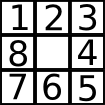
\includegraphics[width=0.40\textwidth]{8pfinal}
    \caption{8 puzzle, estado final}
    \label{fig:8pfinal}
  \end{subfigure}
  \caption{8-puzzle}\label{fig:8p}
\end{figure}






\question Um quebra-cabeça de peças deslizantes consiste em um tabuleiro unidimensional com 7 espaços, três peças pretas no extremo esquerdo, três peças brancas no extremo direto, e um espaço vazio no meio, figura \ref{fig:bp}.

\begin{figure}[h]
    \centering
    
\includegraphics[width=0.40\textwidth]{bp}
    \caption{Quebra-cabeça de peças deslizantes}
    \label{fig:bp}
\end{figure}

Uma peça pode ser movida para uma casa adjacente, este movimento tem custo 1. Uma peça pode pular uma ou duas peças para um espaço em branco, este movimento tem o custo da quantidade de peças puladas.

O objetivo é ter todas as peças brancas a esquerda de todas as peças pretas, a posição do vazio não é importante.

Defina um espaço de estado para o problema e desenvolva uma heurística de avaliação.





\item Desenvolva uma heurística de avaliação para o jogo da velha.


\end{questions}



\end{document}

